\documentclass[11pt]{article}
\usepackage[english]{babel}
\usepackage[utf8]{inputenc}
\usepackage[dvipsnames]{xcolor}
\usepackage[most]{tcolorbox}
\usepackage[linguistics]{forest}
\usepackage{fancyhdr}
\usepackage{amsmath}
\usepackage{amssymb}
\usepackage{amsfonts}
\usepackage{amstext}
\usepackage{amsmath,amssymb,amsthm, thmtools}
\usepackage{tikz,lipsum,lmodern}
\usepackage{array}
\usepackage{lastpage}
\usepackage{multicol}
\usepackage{tikz-cd}
\usepackage{array}
\usepackage{dirtytalk}
\usepackage{qtree}
\usepackage{framed}
\usepackage[hyperfootnotes=false]{hyperref}
\hypersetup{
colorlinks=true,
linkcolor={mypink}}

\definecolor{mypink}{RGB}{255, 50, 147}
\definecolor{pink}{RGB}{255, 0, 147}

\setlength{\textheight}{9.3in}
\setlength{\topmargin}{-0.7in}
\setlength{\textwidth}{6.5in}
\setlength{\oddsidemargin}{0in}
\setlength{\evensidemargin}{0in}
\setlength{\parskip}{6pt}
\setlength{\parindent}{0pt}

\def\mbb{\mathbb}
\def\mb{\mathbf}
\def\mc{\mathcal}
\def\R{\mbb{R}}
\def\Q{\mbb{Q}}
\def\Z{\mbb{Z}}
\def\C{\mbb{C}}
\def\N{\mbb{N}}
\def\F{\mbb{F}}
\def\T{\mc{T}}
\def\A{\mc{A}}
\def\E{\mbb{E}}
\def\P{\mbb{P}}
\def\X{\mathfrak{X}}
\def\e{\epsilon}
\def\d{\delta}
\def\h{\hbar}
\def\w{\omega}
\def\l{\ell}
\def\Ra{\Rightarrow}
\def\La{\Leftarrow}
\def\and{\quad \text{and} \quad}
\def\la{\langle}
\def\ra{\rangle}
\def\sp{\vspace{3mm}}

\def\nemt{\neq \emptyset}
\newcommand{\dif}[2]{\frac{d#1}{d#2}}
\newcommand{\pardif}[2]{\frac{\partial #1}{\partial #2}}
\newcommand{\twopardif}[2]{\frac{\partial ^2 #1}{\partial #2^2}}
\newcommand{\Matrix}[1]{\begin{pmatrix} #1 \end{pmatrix}}
\newcommand{\Lint}[1]{\ointctrclockwise_{#1}}
\newcommand{\Ang}[1]{\left\langle #1 \right\rangle}
\newcommand{\Inn}{\langle \cdot , \cdot \rangle}
\newcommand{\norm}[1]{\left\| #1 \right\|}
\newcommand{\blanknorm}[1]{\| \cdot \|_{#1}}
\newcommand{\epfrac}[1]{\frac{\e}{#1}}
\newcommand{\ext}[1]{\tilde{\mb #1}}

\renewcommand{\epsilon}{\varepsilon}
\renewcommand{\bar}{\overline} 
\renewcommand{\hat}{\widehat}


\declaretheoremstyle[
  headfont=\color{mypink}\normalfont\bfseries,
%  bodyfont=\color{red}\normalfont\itshape,
]{pink}

\declaretheoremstyle[
  headfont=\color{black}\normalfont\bfseries,
%  bodyfont=\color{red}\normalfont\itshape,
]{boxedsolution}

\theoremstyle{pink}
\newtheorem{definition}{Definition}[section]

\theoremstyle{boxedsolution}
\newtheorem*{bproof}{Proof}
\newtheorem*{solution}{Solution}
  
\theoremstyle{definition}
\newtheorem{lemma}[definition]{Lemma}
\newtheorem{theorem}[definition]{Theorem}
\newtheorem{corollary}[definition]{Corollary}
\newtheorem{proposition}[definition]{Proposition}
\newtheorem{example}[definition]{Example}
\newtheorem{problem}{Problem}
\newtheorem{question}{Question}
\newtheorem{Goal}{Goal}

\newtheoremstyle{claim}
{\topsep}{\topsep}{}{}%              
{\bfseries}{:}%             
{5pt plus 1pt minus 1pt}{}%             
\theoremstyle{claim}
% change this to \newtheorem*{claim}{Claim} to leave things un-numbered
\newtheorem{claim}{Claim}



\newenvironment{boxsol}
    {\begin{framed}
    \begin{solution}
    }
    {
    \end{solution}    
    \end{framed}}
    
\newenvironment{boxproof}
    {\begin{framed}
    \begin{bproof}
    }
    {
    \end{bproof}    
    \end{framed}}

\pagestyle{fancy}
\fancyhf{}
\lhead{JCP322 - Assignment 1}
\rhead{Maxim Piatine (1005303100)}
\cfoot{Page \thepage \ of \pageref{LastPage}}

\begin{document}
 \Section*{Question 1}
Eigenstates have a definite kinetic and potential energy, $\hat{H}|\psi\ra=E|\psi\ra$ where the Hamiltonian $\hat{H}$ is denoted by the kinetic and potential energy $\hat{H}=\hat{T}+\hat{V}=\frac{\hat{p}^2}{2m}+\frac{1}{2}m\w^2\hat{x}^2$, the energy $E$ which is an eigenvalue of the Hamiltonian operator in other words its just a value, and the eigenstate $|\psi\ra$ denotes the energy level, the Hamiltonian is an operator that acts on the states of the system. That concludes, that there is a kinetic and potential energy involved in our eigenstate. The definite comes from the eigenstate, on a quantum mechanical harmonic oscillator, we can see that each energy level acquired is set by the formula $E_n=(n+\frac{1}{2})\h\w$, which can be shown on the graph below, and $x$ is just the position. The big parabola surrounding the graph is the potential energy and essentially the borders. Each increment of energy levels increase the potentially energy which then also increases the perturbation of $\psi(x)$. Meaning, there is kinetic energy present in the system since wave functions are consisted of potential and kinetic energy. Also, there is more movement on the displacement axis when going up the dependent axis; meaning, more momentum. 
\begin{center}
    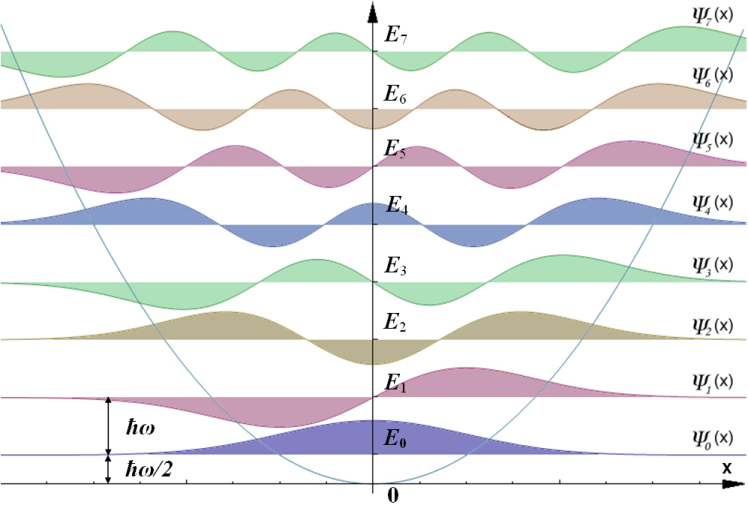
\includegraphics[width=12cm]{harmosc.png}\\
    source: \url{https://qsm.quantumtinkerer.tudelft.nl/4_ZPFs/}
\end{center}
This can also be solved with the annihilation and creation operator. We know that there is a ground state at $E_0$ which is also represented as $\hat{a}^+|\psi_0\ra=|\psi_{1}\ra$ since there is no other direction but up the ladder because there is nothing lower than the ground state. The higher we increase the creation operator the higher the energy levels become, hence the formula $\hat{a}^+|\psi_0\ra=\sqrt{n+1}|\psi_{n+1}\ra$. The same goes for the annihilation operator which decreases the energy level going down until the ground state.
\newpage
 \section*{Question 2}
 Let $1$ be the unit operator.
 (a)\[\la Q\ra=\la\psi|\hat{Q}|\psi\ra=\la\psi|1\hat{Q}1|\psi\ra=\int^\infty_{-\infty}\int^\infty_{-\infty}dxdx'
 \la\psi|x\ra \la x|\hat{Q}|x'\ra \la x'|\psi\ra\]
 \sp
 \\Facts: $\hat{Q}|x\ra=Q|x\ra$, $\la \psi|x\ra=\la x|\psi\ra^*$, $\la x|\psi\ra=\psi(x)$ 
 \sp
 \[=\int^\infty_{-\infty}\int^\infty_{-\infty}\la x|\psi\ra^*\la x|Q|x'\ra \la x'|\psi\ra dxdx'=\int^\infty_{-\infty}\psi(x)^*Q\psi(x)dx=\int^\infty_{-\infty}|\psi(x)|^2Qdx\]
 (b)
\[\la X\ra=\la\psi|\hat{X}|\psi\ra=\la\psi|1\hat{X}1|\psi\ra=\int^\infty_{-\infty}\int^\infty_{-\infty}dxdx'
 \la\psi|x\ra \la x|\hat{X}|x'\ra \la x'|\psi\ra\]
 \sp
 \\Facts: $\hat{X}|x\ra=x|x\ra$, $\la x|x'\ra=\delta_{x,x'}$(reduces double integral into single integral), $\la \psi|x\ra=\la x|\psi\ra^*$, $\la x|\psi\ra=\psi(x)$ 
 \sp
 \[=\int^\infty_{-\infty}\int^\infty_{-\infty}\la x|\psi\ra^*\la x|x|x'\ra \la x'|\psi\ra dxdx'=
 \int^\infty_{-\infty}\int^\infty_{-\infty}\la x|\psi\ra^*x'\la x|x'\ra \la x'|\psi\ra dxdx'
 \]
 \sp
 \[=\int^\infty_{-\infty}\int^\infty_{-\infty}\la x|\psi\ra^*x'\delta_{x,x'} \la x'|\psi\ra dxdx'=
 \int^\infty_{-\infty}\psi(x)^*x\psi(x)dx=\int^\infty_{-\infty}x|\psi(x)|^2dx\]
 
\newpage
 \section*{Question 3}
(a)
\[\hat{H}^{(0)}=\Matrix{1 & 0 & 0\\ 0 & 3 & 0\\ 0 & 0 & -2}, \delta\hat{H}=\Matrix{0 & 0 & V\\ 0 & V & 0\\ V & 0& 0}\]
\sp
\[\hat{H}(\lambda)=\hat{H}^{(0)}+\lambda\delta\hat{H}=  \Matrix{1 & 0 & 0\\ 0 & 3 & 0\\ 0 & 0 & -2}+ \lambda\Matrix{0 & 0 & V\\ 0 & V & 0\\ V & 0& 0}= \Matrix{1 & 0 & V\lambda\\ 0 & 3+V\lambda & 0 \\ V\lambda & 0 & -2}\]
Since perturbation has been turned on we state that $\lambda = 1$.
\sp
\[\hat{H}(\lambda)=\Matrix{1 & 0 & V \\ 0 & 3+V & 0\\ V & 0 & -2}\]
\sp
\[det\left(\hat{H}(\lambda)-\alpha I\right)=det \left(\Matrix{1 & 0 & V \\ 0 & 3+V & 0\\ V & 0 & -2} - \Matrix{\alpha & 0 & 0\\ 0 & \alpha & 0\\ 0 & 0 & \alpha}\right)=det \Matrix{ 1-\alpha & 0 & V\\ 0 & 3+V-\alpha & 0\\ V & 0 & -2-\alpha}=0\]
\sp
\[=(1-\alpha)\begin{vmatrix} 3 + V -\alpha & 0\\ 0 & -2 -\alpha\end{vmatrix}+V\begin{vmatrix} 0 & 3+V-\alpha\\ V & 0\end{vmatrix}
=(1-\alpha)(3+V-\alpha)(-2-\alpha)-V(V)(3+V-\alpha)\]
\sp
\[=(1-\alpha)(3+V-\alpha)(-2-\alpha)-V(V)(3+V-\alpha)=-\alpha^3+\alpha^2(2+V)+\alpha(5+V+V^2)-(6+2V+3V^2+V^3)=0\]
In order to solve the cubic, we can guess one of the roots, which in this case is $V+3$, From there we can do synthetic/long division to find the remaining quadratic term (this is fully done on rough paper attached below):
\sp
\[\frac{-\alpha^2+2\alpha^2+V\alpha^2+5\alpha+V\alpha+V^2\alpha-6-2V-3V^2-V^3}{\alpha-3-a}=-\alpha^2-\alpha+2+V^2\]
From the remaining quadratic term, we can use the quadratic formula:
\sp
\[\alpha_{1,2}=\frac{1\pm\sqrt{1-4(-1)(2+V^2)}}{2(-1)}=\frac{-1\pm\sqrt{4V^2+9}}{2}\]
\sp
\[\alpha_3=3+V\]
The eigenvalues are represented by $\alpha_{1,2,3}$.
\newpage
(b)
Unperturbed Energy
\sp
\[\hat{H}^{(0)}=\Matrix{1 & 0 & 0\\ 0 & 3 & 0\\ 0 & 0 & -2}\]
\sp
\[E^{(0)}_0=1 \text{ } \text{ , } \text{ } E^{(0)}_1=3  \text{ } \text{ , } \text{ } E^{(0)}_2=-2\]
\sp % this is wtv
\[\delta\hat{H}=\Matrix{0 & 0& V\\ 0 & V & 0\\ V & 0 & 0}=\Matrix{\la0|\delta\hat{H}|0\ra & \la0|\delta\hat{H}|1\ra & \la0|\delta\hat{H}|2\ra \\ \la1|\delta\hat{H}|0\ra & \la1|\delta\hat{H}|1\ra & \la1|\delta\hat{H}|2\ra\\
\la2|\delta\hat{H}|0\ra & \la2|\delta\hat{H}|1\ra & \la2|\delta\hat{H}|2\ra }\]
\sp
\[E_n^{(1)}= \la n^{(0)}|\delta \hat{H}|n^{(0)}\ra\]
\sp
\[E_0^{(1)}= \la 0|\delta\hat{H}|0 \ra= 0 \text{ } \text{ , } \text{ } E_1^{(1)}= \la 1|\delta\hat{H}|1 \ra= V \text{ } \text{ , } \text{ } E_2^{(1)}= \la 2|\delta\hat{H}|2 \ra= 0\]
\sp
\[E_n^{(2)}= \sum_{k\neq n}\frac{|\la k^{(0)}|\delta \hat{H}|n^{(0)}\ra|^2}{E_n^{(0)}-E_k^{(0)}}\]
\sp
\[E_0^{(2)}=\sum_{k\neq n}\frac{|\la k^{(0)}|\delta \hat{H}|0\ra|^2}{E_0^{(0)}-E_k^{(0)}}=\frac{|\la 1|\delta \hat{H}|0\ra|^2}{E_0^{(0)}-E_1^{(0)}}+\frac{|\la 2|\delta \hat{H}|0\ra|^2}{E_0^{(0)}-E_2^{(0)}}=0+\frac{V^2}{1-(-2)}=\frac{V^2}{3}\]
\sp
\[E_1^{(2)}=\sum_{k\neq n}\frac{|\la k^{(0)}|\delta \hat{H}|1\ra|^2}{E_1^{(0)}-E_k^{(0)}}=
\frac{|\la 0|\delta \hat{H}|1\ra|^2}{E_1^{(0)}-E_0^{(0)}}+
\frac{|\la 2|\delta \hat{H}|1\ra|^2}{E_1^{(0)}-E_2^{(0)}}
=0\]
\sp
\[E_2^{(2)}=\sum_{k\neq n}\frac{|\la k^{(0)}|\delta \hat{H}|2\ra|^2}{E_2^{(0)}-E_k^{(0)}}=
\frac{|\la 0|\delta \hat{H}|2\ra|^2}{E_2^{(0)}-E_0^{(0)}}+
\frac{|\la 1|\delta \hat{H}|2\ra|^2}{E_2^{(0)}-E_1^{(0)}}
=\frac{V^2}{-2-1}+0=-\frac{V^2}{3}\]
\sp
\[E_0=E_0^{(0)}+E_0^{(1)}+E_0^{(2)}=1+0+\frac{V^2}{3}=1+\frac{V^2}{3}\]
\sp
\[E_1=E_1^{(0)}+E_1^{(1)}+E_1^{(2)}=3+V\]
\sp
\[E_2=E_2^{(0)}+E_2^{(1)}+E_2^{(2)}=-2+0-\frac{V^2}{3}=-2-\frac{V^2}{3}\]
\newpage
(c) if we take V to be significantly small $V\ll 1$, we can assume $V=0$:
\sp
\\Take the calculated energy corrections from (b)
\[E_0\approx 1+0=1 \text{ } \text{ , } \text{ } E_1\approx3+0=3 \text{ } \text{ , } \text{ } E_2 \approx -2 - 0 = -2\]
\sp
\\and the eigenvalues from (a):
\[\alpha_1\approx\frac{-1+\sqrt{9}}{2}=\frac{-1+3}{2}=1 \text{ } \text{ , } \text{ } \alpha_2\approx\frac{-1-\sqrt{9}}{2}=\frac{-1-3}{2}=-2 \text{ } \text{ , } \text{ }
\alpha_3 \approx 3+0 = 3\]
Therefore, the results in (a) and in (b) would make the perturbation theory valid under the condition that $V=0$, $V\ll1$.
Proving the validity we need to use the Taylor series expansion. 
\sp
\[f(x)=\sqrt{1+x^2}=1+\frac{x^2}{2}+\frac{x^4}{8}+\frac{x^6}{16}+\dots\]
\sp
\\Take $\sqrt{4V^2+9}$ which is the discriminant of the quadratic formula obtained while finding the eigenvalues. 
\sp
\[f(V)=f(a)+\frac{f'(a)}{1!}(V-a)+\frac{f''(a)}{2!}(V-a)^2\]
\sp
Let $a=0$:
\sp
\[f(V)=f(0)+\frac{f'(0)}{1!}(V-0)+\frac{f''(0)}{2!}(V-0)^2\]
\sp
\[=\sqrt{4(0)+9}+\frac{8(0)}{2\sqrt{4(0)+9}}(V)+\frac{36}{2!(4(0)+9)^{3/2}}(V^2)=3+0+\frac{2}{3}V^2=3+\frac{2}{3}V^2\]
\sp
\\Therefore, after replacing the discriminant by the Taylor expansion on the eigenvalues $\alpha_{1,2}$ you can see they are the same as the energies in (b).


\newpage
 \section*{Question 4}
(a)
\[\delta\hat{H}=\alpha\hat{X}^3\]
Let $1$ be the unit operator.
\sp
\[E_n^{(1)}=\la \psi_n^{(0)}|\delta \hat{H}|\psi_n^{(0)}\ra = 
\la \psi_n^{(0)}|1 \delta \hat{H} 1|\psi_n^{(0)}\ra  \]
\sp
\begin{tcolorbox}
Useful Facts:
\sp
\[1 = \int^\infty_{-\infty}|x\ra\la x|dx\]
\sp
\[\la \psi^{(0)}_n|x\ra = \psi_n(x)=\sqrt{\frac{2}{a}}\sin{\left(\frac{n\pi x}{a}\right)}\]
\sp
\[\delta\hat{H}|x\ra=\delta H |x\ra\]
\end{tcolorbox}
\[=\int^\infty_{-\infty}\int^\infty_{-\infty}dxdx'\la \psi_n^{(0)}|x\ra \la x |\delta \hat{H}|x\ra\la x|\psi_n^{(0)}\ra=\int^\infty_{-\infty}\psi_n^{(0)*}\delta H\psi_n^{(0)}dx=
\int^\infty_{-\infty}\left(\sqrt{\frac{2}{a}}\sin\left(\frac{n\pi x}{a}\right)\right)^2\delta Hdx\]
\sp
\[=\int^\infty_{-\infty}\frac{2}{a}\sin^2\left(\frac{n\pi x}{a}\right)\left(\alpha\hat{x}^3\right)dx
=\frac{2\alpha}{a}\int^{\infty}_{-\infty}x^3\sin^2\left(\frac{n\pi x}{a}\right)dx\]
\sp
\\We know that $x^3$ is an odd function and $\sin^2(x)$ is an even function. An odd function times and even function becomes an odd function. Due to symmetry of $-\infty$ and $\infty$ the integral of an odd function is zero.
\[E_n^{(1)}=\frac{2\alpha}{a}\int^{\infty}_{-\infty}x^3\sin^2\left(\frac{n\pi x}{a}\right)dx=0\]
\sp
Another way, of doing it is expanding the position operator:
\[\hat{X}=\sqrt{\frac{\h}{2m\w_0}}\left(\hat{a}^++\hat{a}\right) \text{  } \Rightarrow \text{ } \hat{X}^3=\left(\frac{\h}{2m\w_0}\right)^{3/2}\left(\hat{a}^++\hat{a}\right)^3\]
\sp
\[\hat{X}^3=\left(\frac{\h}{2m\w_0}\right)^{3/2}\left(\hat{a}^{+3}+\hat{a}^{+}\hat{a}\hat{a}^{+}+\hat{a}\hat{a}^{+2}+\hat{a}^{2}\hat{a}^{+}+\hat{a}^{+2}\hat{a}+\hat{a}^{+}\hat{a}^{2}+\hat{a}\hat{a}^{+}\hat{a}+\hat{a}^{3}\right)\]
\sp
\[E_n^{(1)}=\la n'|\delta \hat{H}|n\ra = \la n'|\alpha \hat{X}^3|n\ra = \alpha\Bigg\la n'\Bigg|\left(\frac{\h}{2m\w_0}\right)^{3/2}\left(\hat{a}^++\hat{a}\right)^3\Bigg|n\Bigg\rangle \]
\sp
\[= \alpha\left(\frac{\h}{2m\w_0}\right)^{3/2}\Big\la n'\Big|\left(\hat{a}^++\hat{a}\right)^3\Big|n\Big\ra\]
\newpage
\[
\begin{cases}
(1) \text{ } \la n\text{ }|\hat{a}^{+}\text{ }\hat{a}^{+}\text{ }\hat{a}^{+}|\text{ }n\ra=\sqrt{(n+1)(n+2)(n+3)}\la n\text{ }|\text{ }n+3\ra
\sp
\\(2) \text{ } \la n\text{ }|\hat{a}\text{ }\hat{a}\text{ }\hat{a}|\text{ }n\ra=\sqrt{n(n-1)(n-2)}\la n\text{ }|\text{ }n-3\ra
\sp
\\(3)  \text{ } \la n\text{ }|\hat{a}^{+}\text{ }\hat{a}\text{ }\hat{a}^{+}|\text{ }n\ra=\sqrt{(n+1)^3}\la n\text{ }|\text{ }n+1\ra
\sp
\\(4)   \text{ } \la n\text{ }|\hat{a}\text{ }\hat{a}^{+}\text{ }\hat{a}|\text{ }n\ra=\sqrt{n^3}\la n\text{ }|\text{ }n-1\ra
\sp
\\(5)   \text{ } \la n\text{ }|\hat{a}\text{ }\hat{a}^{+}\text{ }\hat{a}^{+}|\text{ }n\ra=\sqrt{(n+1)(n+2)^2}\la n\text{ }|\text{ }n+1\ra
\sp
\\(6)   \text{ } \la n\text{ }|\hat{a}^{+}\text{ }\hat{a}\text{ }\hat{a}|\text{ }n\ra=\sqrt{n(n-1)^2}\la n\text{ }|\text{ }n-1\ra
\sp
\\(7)   \text{ } \la n\text{ }|\hat{a}\text{ }\hat{a}\text{ }\hat{a}^{+}|\text{ }n\ra=\sqrt{(n+1)^2n}\la n\text{ }|\text{ }n-1\ra
\sp
\\(8)   \text{ } \la n\text{ }|\hat{a}^{+}\text{ }\hat{a}^{+}\text{ }\hat{a}|\text{ }n\ra=\sqrt{n^2(n+1)}\la n\text{ }|\text{ }n+1\ra
\end{cases}\]
With the possible of 8 cases, all of them are with the right combinations are orthogonal to one another. making the total summation equal to zero.
\sp
\[E_n^{(1)}=\alpha\left(\frac{\h}{2m\w_0}\right)^{3/2}\la n'| 0 | n \ra = 0\]
Therefore, the first-order correction to the energy of the harmonic oscillator are:
\sp
\[E_n\approx E_n^{(0)}+E_n^{(1)}=\frac{n^2\pi^2\h^2}{2ma^2}+0=\frac{n^2\pi^2\h^2}{2ma^2}\]
(b)
\[E_n^{(2)}=\sum_{k\neq n}\frac{| \delta \hat{H}_{k,n}|^2}{E^{(0)}_n-E^{(0)}_k}\]
\sp
\[
\delta \hat{H}_{k,n}=\la k|\delta\hat{H}| n\ra= \la k|\alpha \hat{X}^3| n\ra= \alpha\la k|\hat{X}^3| n\ra=
\alpha\left(\frac{\h}{2m\w_0}\right)^{3/2}\la k|\left(\hat{a}^++\hat{a}\right)^3| n\ra
\]
\sp
\\With the combinations I shown in (a) we can substitute the bra with $k$ and transform the braket to $\delta_{k,n}$.
\sp
\[\la k|\left(\hat{a}^++\hat{a}\right)^3| n\ra = \sqrt{(n+1)(n+2)}(n+3)\delta_{k,n+3} + \sqrt{n(n-1)(n-2)}\delta_{k,n-3}+
\dots\]
\sp
\[\dots + \sqrt{n+1}((n+1)+(n+2)+n)\delta_{k,n+1}+\sqrt{n}((n+(n-1)+(n+1)))\delta_{k,n-1}\]
\sp
\[=\sqrt{(n+1)(n+2)(n+3)}\delta_{k,n+3} + 
\sqrt{n(n-1)(n-2)}\delta_{k,n-3}+
3(n+1)^{3/2}\delta_{k,n+1}+
3n^{3/2}\delta_{k,n-1}\]


\newpage
%%Wait to use this
\[E_n^{(2)}=\alpha^2\left(\frac{\h}{2m\w_0}\right)^{3}\Bigg[
(n+1)(n+2)(n+3)\sum_{k\neq n}\frac{|\delta_{k,n+3}|^2}{E^{(0)}_n-E^{(0)}_k} 
+ n(n-1)(n-2)\sum_{k\neq n}\frac{|\delta_{k,n-3}|^2}{E^{(0)}_n-E^{(0)}_k} + \dots
\]
\sp
\[\dots +9(n+1)^3\sum_{k\neq n}\frac{|\delta_{k,n+1}|^2}{E^{(0)}_n-E^{(0)}_k}
+ 9n^3\sum_{k\neq n}\frac{|\delta_{k,n-1}|^2}{E^{(0)}_n-E^{(0)}_k}\Bigg]
\]
\sp
\[=(\dots)\Bigg[
\frac{(n+1)(n+2)(n+3)}{E^{(0)}_n-E^{(0)}_{n+3}} 
+ \frac{n(n-1)(n-2)}{E^{(0)}_n-E^{(0)}_{n-3}}
+\frac{9(n+1)^3}{E^{(0)}_n-E^{(0)}_{n+1}}
+\frac{9n^3}{E^{(0)}_n-E^{(0)}_k}\Bigg]\]

\sp
\[E^{(0)}_{n}-E^{(0)}_{n+3}=\left(n+\frac{1}{2}\right)\h\w_0-\left(n+\frac{7}{2}\right)\h\w_0=-3\h\w_0\]
\sp
\[E^{(0)}_{n}-E^{(0)}_{n-3}=\left(n+\frac{1}{2}\right)\h\w_0-\left(n-\frac{5}{2}\right)\h\w_0=3\h\w_0\]
\sp
\[E^{(0)}_{n}-E^{(0)}_{n+1}=\left(n+\frac{1}{2}\right)\h\w_0-\left(n+\frac{1}{2}\right)\h\w_0=-\h\w_0\]
\sp
\[E^{(0)}_{n}-E^{(0)}_{n-1}=\left(n+\frac{1}{2}\right)\h\w_0-\left(n-\frac{1}{2}\right)\h\w_0=\h\w_0\]
\sp
\[E^{(2)}_n=\alpha^2\left(\frac{\h}{2m\w_0}\right)^{3}\Bigg[
\frac{(n+1)(n+2)(n+3)}{-3\h\w_0} 
+ \frac{n(n-1)(n-2)}{3\h\w_0}
+\frac{9(n+1)^3}{-\h\w_0}
+\frac{9n^3}{\h\w_0}\Bigg]\]
\sp
\[=\frac{\alpha^2\h^2}{8m^3\w_0^4}(-30n^2-30n-11)=-\frac{\alpha^2\h^2}{8m^3\w_0^4}(30n^2+30n+11)=E^{(2)}_n\]
\sp
\[E_n\approx E_n^{(0)}+E_n^{(1)}+E_n^{(2)}=\frac{n^2\pi^2\h^2}{2ma^2}+0-\frac{\alpha^2\h^2}{8m^3\w_0^4}(30n^2+30n+11)=\frac{n^2\pi^2\h^2}{2ma^2}-\frac{\alpha^2\h^2}{8m^3\w_0^4}(30n^2+30n+11)\]

For the validity of the correction, perturbations must be small and thus if $n$ goes to infinity the correction is no longer valid because the second-order correction to the energy will be infinitely large. 
\newpage
(c) 
\[|n^{(1)}\ra = \sum_{k\neq n} \left(\frac{\delta\hat{H}_{kn}}{E_n^{(0)}-E_k^{(0)}}\right)|k^{(0)}\ra\]
\sp
Using the $\delta \hat{H}_{kn}$ from part b:
\sp
\[\delta\hat{H}_{k,n}=\left(\sqrt{(n+1)(n+2)(n+3)}\delta_{k,n+3} + 
\sqrt{n(n-1)(n-2)}\delta_{k,n-3}+
3(n+1)^{3/2}\delta_{k,n+1}+
3n^{3/2}\delta_{k,n-1}\right)\]
\[=\alpha\left(\frac{\h}{2m\w_0}\right)^{3/2} 
\Bigg[\sqrt{(n+1)(n+2)(n+3)}\sum_{k\neq n}\frac{\delta_{k,n+3}}{E_n^{(0)}-E_k^{(0)}}|k^{(0)}\ra + 
\sqrt{n(n-1)(n-2)}\sum_{k\neq n}\frac{\delta_{k,n-3}}{E_n^{(0)}-E_k^{(0)}}|k^{(0)}\ra 
+ \dots\]
\sp
\[\dots+
3(n+1)^{3/2}\sum_{k\neq n}\frac{\delta_{k,n+1}}{E_n^{(0)}-E_k^{(0)}}|k^{(0)}\ra+ 
3(n)^{3/2}\sum_{k\neq n}\frac{\delta_{k,n-1}}{E_n^{(0)}-E_k^{(0)}}|k^{(0)}\ra\Bigg]\]
\sp
\\Using the same combination of $E_n^{(0)}-E_{n+3}^{(0)}$, $E_n^{(0)}-E_{n-3}^{(0)}$, $E_n^{(0)}-E_{n+1}^{(0)}$, $E_n^{(0)}-E_{n-1}^{(0)}$. We can replace the denominator values by their calculated values from part (b):
\sp
\[=\alpha\left(\frac{\h}{2m\w_0}\right)^{3/2}\Bigg[\frac{\sqrt{(n+1)(n+2)(n+3)}}{-3\h\w_0}|n^{(0)}+3\ra
+\frac{3(n+1)^{3/2}}{-\h\w_0}|n^{(0)}+1\ra+\dots\]
\sp
\[\dots+
\frac{3n^{3/2}}{\h\w_0}|n^{(0)}-1\ra+
\frac{\sqrt{n(n-1)(n-2)}}{3\h\w_0}|n^{(0)}-3\ra\]
\sp
Let $\beta=\alpha\left(\frac{\h}{2m\w_0}\right)^{3/2}$:
\sp
\[|n^{(1)}\ra=\beta\Bigg[-\frac{\sqrt{(n+1)(n+2)(n+3)}}{3\h\w_0}|n^{(0)}+3\ra
-\frac{3(n+1)^{3/2}}{\h\w_0}|n^{(0)}+1\ra+\frac{3n^{3/2}}{\h\w_0}|n^{(0)}-1\ra+\dots
\]
\sp
\[\dots+\frac{\sqrt{n(n-1)(n-2)}}{3\h\w_0}|n^{(0)}-3\ra\Bigg]\]
\[\mathbb{1}\]

\end{document}
